\documentclass[11pt]{beamer}\usepackage[]{graphicx}\usepackage[]{color}
%% maxwidth is the original width if it is less than linewidth
%% otherwise use linewidth (to make sure the graphics do not exceed the margin)
\makeatletter
\def\maxwidth{ %
  \ifdim\Gin@nat@width>\linewidth
    \linewidth
  \else
    \Gin@nat@width
  \fi
}
\makeatother

\definecolor{fgcolor}{rgb}{1, 1, 0.941}
\newcommand{\hlnum}[1]{\textcolor[rgb]{0.804,0.718,0.71}{#1}}%
\newcommand{\hlstr}[1]{\textcolor[rgb]{0.604,0.753,0.804}{#1}}%
\newcommand{\hlcom}[1]{\textcolor[rgb]{0.439,0.502,0.565}{#1}}%
\newcommand{\hlopt}[1]{\textcolor[rgb]{1,1,0.941}{#1}}%
\newcommand{\hlstd}[1]{\textcolor[rgb]{1,1,0.941}{#1}}%
\newcommand{\hlkwa}[1]{\textcolor[rgb]{0.941,0.902,0.549}{#1}}%
\newcommand{\hlkwb}[1]{\textcolor[rgb]{1,0.871,0.678}{#1}}%
\newcommand{\hlkwc}[1]{\textcolor[rgb]{0.545,0.941,0.702}{#1}}%
\newcommand{\hlkwd}[1]{\textcolor[rgb]{0.545,0.941,0.902}{#1}}%
\let\hlipl\hlkwb

\usepackage{framed}
\makeatletter
\newenvironment{kframe}{%
 \def\at@end@of@kframe{}%
 \ifinner\ifhmode%
  \def\at@end@of@kframe{\end{minipage}}%
  \begin{minipage}{\columnwidth}%
 \fi\fi%
 \def\FrameCommand##1{\hskip\@totalleftmargin \hskip-\fboxsep
 \colorbox{shadecolor}{##1}\hskip-\fboxsep
     % There is no \\@totalrightmargin, so:
     \hskip-\linewidth \hskip-\@totalleftmargin \hskip\columnwidth}%
 \MakeFramed {\advance\hsize-\width
   \@totalleftmargin\z@ \linewidth\hsize
   \@setminipage}}%
 {\par\unskip\endMakeFramed%
 \at@end@of@kframe}
\makeatother

\definecolor{shadecolor}{rgb}{.97, .97, .97}
\definecolor{messagecolor}{rgb}{0, 0, 0}
\definecolor{warningcolor}{rgb}{1, 0, 1}
\definecolor{errorcolor}{rgb}{1, 0, 0}
\newenvironment{knitrout}{}{} % an empty environment to be redefined in TeX

\usepackage{amsmath}
\usepackage{alltt}

%=======================================================================
% General packages
\usepackage[british]{babel}
\usepackage[T1]{fontenc}
\usepackage[utf8]{inputenc}
\usepackage{lmodern}
\usepackage{multicol}
\usepackage{mathtools} %% Funcionalidades (como \dcases)
\usepackage{dsfont}    %% Para \mathds{1} Indicadora
\usepackage{bm}

%=======================================================================
% For figures
\usepackage{graphicx}
\usepackage[export]{adjustbox}

%% ======================================================================
%% Fontes
\usepackage{mathpazo}
\usepackage{inconsolata}
\usepackage{verbatim}

\usefonttheme{professionalfonts}
\usefonttheme{serif}

%=======================================================================
% For tables
\usepackage[bottom]{footmisc}
\usepackage{booktabs}
\usepackage{threeparttable}
\usepackage{tabularx}
\usepackage{makecell}
\usepackage{colortbl}
\newcolumntype{C}{>{\centering\arraybackslash}X}
\newcolumntype{L}[1]{>{\raggedright\let\newline\\\arraybackslash\hspace{0pt}}m{#1}}
\DeclareRobustCommand{\rchi}{{\mathpalette\irchi\relax}}
\newcommand{\irchi}[2]{\raisebox{\depth}{$#1\chi$}}
\usepackage{float}
\makeatletter
\def\@xfootnote[#1]{%
  \protected@xdef\@thefnmark{#1}%
  \@footnotemark\@footnotetext}
\makeatother

%=======================================================================
% For captions
\usepackage{caption}
\captionsetup{
  justification=raggedright,
  singlelinecheck=false,
  font=footnotesize
}

%% ======================================================================
%% Cores para links
\definecolor{url}{HTML}{000080}
\definecolor{run}{HTML}{4A0082}
\definecolor{col}{HTML}{6180A6}
\usepackage{hyperref}
\hypersetup{colorlinks, allcolors=., urlcolor=url, runcolor=run}

%\setbeamercolor{bibliography entry author}{fg=black}
%\usepackage[alf]{abntex2cite}
\usepackage{natbib}
\bibliographystyle{agsm}

%=======================================================================
% Algorithms
\usepackage[english, vlined, ruled]{algorithm2e}
\SetAlCapSty{}
\SetAlCapFnt{\footnotesize\color{col}}
\SetAlCapNameFnt{\footnotesize}

% Customize captions styles
\usepackage{caption}
\captionsetup{
  font=footnotesize,
  labelfont={color=col}
}

%% ======================================================================
%% Tema e cores do documento
\usetheme{CambridgeUS}
\setbeamertemplate{itemize items}[triangle]
\setbeamertemplate{enumerate items}[default]
\setbeamertemplate{navigation symbols}{}

\setbeamertemplate{frametitle}{
  \nointerlineskip
  \begin{beamercolorbox}[sep=0.3cm, ht=1.8em,
    wd=\paperwidth]{frametitle}
    \vbox{}\vskip-2ex%
    \strut\hspace*{3ex}\Large\bfseries\insertframetitle\strut
    \vskip-0.8ex%
  \end{beamercolorbox}
}

%% Slides em geral
\setbeamercolor{frametitle}{bg=white, fg=col}
\setbeamercolor{structure}{fg=col}
\setbeamercolor{palette primary}{bg=gray!30, fg=col}
\setbeamercolor{palette tertiary}{bg=col, fg=white}
\setbeamercolor{footlinecolor}{fg=white,bg=col}
\setbeamercolor{caption name}{fg=col}

% \setbeamertemplate{frametitle continuation}{[\insertcontinuationcount]}
\setbeamertemplate{frametitle continuation}{}

%% Slide Inicial
\setbeamertemplate{title page}[default]
\setbeamercolor{title}{fg=col}
\setbeamercolor{author}{fg=black!70}
\setbeamercolor{institute}{fg=black!70}
\setbeamercolor{date}{fg=black!70}
\setbeamerfont{title}{series=\bfseries, size=\Large}

%% ======================================================================
%% Definição do cabeçalho e rodapé
\setbeamerfont{headline}{size=\fontsize{5}{5}\selectfont}
\setbeamertemplate{headline}{\bfseries
  \leavevmode%
  \hbox{%
    \begin{beamercolorbox}[wd=.5\paperwidth, ht=2.2ex, dp=1ex, right,
      rightskip=1em]{section in head/foot}
      \hspace*{2ex}\insertsectionhead
    \end{beamercolorbox}%
    \begin{beamercolorbox}[wd=.5\paperwidth, ht=2.2ex, dp=1ex, left,
      leftskip=1em]{subsection in head/foot}
      \insertsubsectionhead\hspace*{2ex}
    \end{beamercolorbox}}
  \vskip0pt
}

\setbeamerfont{footline}{size=\fontsize{5}{5}\selectfont}
\makeatletter
\setbeamertemplate{footline}{\bfseries
  \leavevmode%
  \hbox{%
    \begin{beamercolorbox}[wd=.3\paperwidth, ht=2.4ex, dp=1ex, right,
      rightskip=1em]{footlinecolor}
      \centering \insertshortauthor%
    \end{beamercolorbox}%
    \begin{beamercolorbox}[wd=.6\paperwidth, ht=2.4ex, dp=1ex, left,
      leftskip=1em]{footlinecolor}
      \hfill\insertshorttitle%
    \end{beamercolorbox}%
    \begin{beamercolorbox}[wd=.1\paperwidth, ht=2.4ex, dp=1ex, left,
      leftskip=1em]{footlinecolor}
      \centering Slide \insertframenumber
    \end{beamercolorbox}}
  \vskip0pt
}
\makeatother

%% ======================================================================
%% Layout do tableofcontents
\setbeamertemplate{section in toc}{
  {\color{col} \bfseries\inserttocsectionnumber.}~
  {\leftskip=0.5em\color{black}\inserttocsection\par}
}

\setbeamertemplate{subsection in toc}{
  {\color{col!80}
  \bfseries\inserttocsectionnumber.\inserttocsubsectionnumber}~
  \leftskip=2em{\color{black}\inserttocsubsection\par}
}

%% ======================================================================
%% Formatando slides para seções e subseções
\AtBeginSection[]{
  \begin{frame}[c, allowframebreaks, noframenumbering]
    \begin{center}
      \textcolor{col}{\thesection} \\ \vspace{0.3cm}
      \parbox{0.6\textwidth}{
        \centering \textcolor{col}{\LARGE \bf \insertsection}}\\
    \end{center}
  \end{frame}
}

\AtBeginSubsection{
  \begin{frame}[c, allowframebreaks, noframenumbering]
    \begin{center}
      \textcolor{col}{\thesection.\thesubsection} \\ \vspace{0.3cm}
      \parbox{0.6\textwidth}{
        \centering \textcolor{col!80}{\large \insertsection}\\
        \centering \textcolor{col}{\Large \bf \insertsubsection}}\\
    \end{center}
  \end{frame}
}

%% ======================================================================
%% Metadados não disponíveis no YAML com o atual default.tex template

\title[Flexible Models for Analysis of Dispersed Count Data]{
  Flexible Models for Analysis of\\ Dispersed Count Data}

\author[Eduardo E. Ribeiro Jr]{
  Eduardo Elias Ribeiro Junior\\
  Advisor: PhD. Clarice Garcia Borges Demétrio
}

\institute{
  University of São Paulo - USP\\
  Luiz de Queiroz College of Agriculture - ESALQ\\
  Graduate Program in Statistics and Agricultural Experimentation
}

\date{\small \today \\[0.2cm]
  \url{jreduardo@usp.br} | \url{edujrrib@gmail.com}}




\IfFileExists{upquote.sty}{\usepackage{upquote}}{}
\begin{document}

\begin{frame}[plain, noframenumbering]
  \titlepage
\end{frame}

\begin{frame}[noframenumbering]{Outline}
  \vspace{-0.5cm}
  \tableofcontents[hideallsubsections]
\end{frame}

\section{Introduction}

\begin{frame}{Motivation}

Count data are frequent in many research areas:
\begin{itemize}
  \item Social and political (number of individuals, votes, etc.),
  \item Entomology and biology science (number of insects, offspring,
    etc.),
  \item Medical science (number of patients, number of spots, etc.),
  \item Environmental and crop sciences (number of pests, animals, etc.).
\end{itemize}
\vspace{0.3cm}

In particular for agricultural experimentation area, we have examples
for:

\begin{itemize}
  \item Pets in soybean culture;
  \item Potassium fertilization in soybean culture;
  \item Artificial defoliation in cotton phenology; and
  \item Whitefly in cotton crop.
\end{itemize}

\end{frame}

\begin{frame}{Poisson model and limitations}

  How to analyse count data?

  \begin{itemize}
    \item[] {\bf GLM framework \citep{Nelder1972}}
    \item Provide suitable distribution for a counting random variables;
    \item Efficient algorithm for estimation and inference;
    \item Implemented in many software.
      \vspace{0.3cm}
    \item[] {\bf Poisson model}
    \item Relationship between mean and variance,
      $\text{E}(Y)=\text{Var}(Y)$;
      \vspace{0.3cm}
    \item[] {\bf Main limitations}
    \item Overdispersion (more common), $\text{E}(Y)<\text{Var}(Y)$;
    \item Underdispersion (less common), $\text{E}(Y)>\text{Var}(Y)$.
  \end{itemize}

\end{frame}

\begin{frame}{Dispersion in the count data}

\begin{knitrout}
\definecolor{shadecolor}{rgb}{0.122, 0.188, 0.282}\color{fgcolor}\begin{figure}[!htb]

{\centering \includegraphics[width=\textwidth]{figure/processo-pontual-1} 

}

\caption[Illustration of a possible generator process for under-, over- and equidispered count data]{Illustration of a possible generator process for under-, over- and equidispered count data.}\label{fig:processo-pontual}
\end{figure}


\end{knitrout}

\end{frame}

\section{Motivating examples}

\begin{frame}{Artificial defoliation in cotton phenology}
\vspace{-0.2cm}
\begin{knitrout}
\definecolor{shadecolor}{rgb}{0.122, 0.188, 0.282}\color{fgcolor}\begin{figure}[!htb]

{\centering \includegraphics[width=\textwidth]{figure/desc-cotton2-1} 

}

\caption[(a) Perfis das contagens de ninfas observadas para cada bloco em cada uma das quatro cultivares BRS, as linhas em preto representam os perfis médios]{(a) Perfis das contagens de ninfas observadas para cada bloco em cada uma das quatro cultivares BRS, as linhas em preto representam os perfis médios. (b) Dispersão das médias (eixo $x$) e variâncias (eixo $y$) amostrais, na escala logarítmica, calculadas sobre os blocos em cada tempo e cultivar para cada variável de interesse, a linha pontilhada representa a reta média $=$ variância (equidispersão) e a contínua representa um ajuste de mínimos quadrados.}\label{fig:desc-cotton2}
\end{figure}


\end{knitrout}

\end{frame}

\begin{frame}{Potassium fertilization on soybean culture}
\vspace{-0.3cm}
\begin{knitrout}
\definecolor{shadecolor}{rgb}{0.122, 0.188, 0.282}\color{fgcolor}\begin{figure}[!htb]

{\centering \includegraphics[width=\textwidth]{figure/desc-soya2-1} 

}

\caption[(a) Perfis das contagens de ninfas observadas para cada bloco em cada uma das quatro cultivares BRS, as linhas em preto representam os perfis médios]{(a) Perfis das contagens de ninfas observadas para cada bloco em cada uma das quatro cultivares BRS, as linhas em preto representam os perfis médios. (b) Dispersão das médias (eixo $x$) e variâncias (eixo $y$) amostrais, na escala logarítmica, calculadas sobre os blocos em cada tempo e cultivar para cada variável de interesse, a linha pontilhada representa a reta média $=$ variância (equidispersão) e a contínua representa um ajuste de mínimos quadrados.}\label{fig:desc-soya2}
\end{figure}


\end{knitrout}

\end{frame}

\begin{frame}{Assessing toxicity of nitrofen in aquatic systems}

\begin{figure}[!htb]

{\centering \includegraphics[width=\textwidth]{figure2/desc-nitrofen-1} 

}

\caption[(a) Number of live offsprings observed for each nitrofen concentration level and (b) scatterplot of the sample means against sample variances]{(a) Number of live offsprings observed for each nitrofen concentration level and (b) scatterplot of the sample means against sample variances.}\label{fig:desc-nitrofen}
\end{figure}



\end{frame}

\begin{frame}{Clinical trial in epileptic patients}

\begin{knitrout}
\definecolor{shadecolor}{rgb}{0.122, 0.188, 0.282}\color{fgcolor}\begin{figure}[!htb]

{\centering \includegraphics[width=\textwidth]{figure/desc-epilepsy2-1} 

}

\caption[(a) Profiles by each block (gray lines) and average profile (black lines)]{(a) Profiles by each block (gray lines) and average profile (black lines). (b) Scatter plot of samples means against sample variances, on the logarithm scale. The dotted line is the identity line (equidispersion) and the continous line is the least squares line.}\label{fig:desc-epilepsy2}
\end{figure}


\end{knitrout}

\end{frame}

\begin{frame}{Alternative substrates for bromelia culture}

\begin{figure}[!htb]

{\centering \includegraphics[width=\textwidth]{figure2/plot-bromelia-1} 

}

\caption[(a) Profiles by each block (gray lines) and average profile (black lines)]{(a) Profiles by each block (gray lines) and average profile (black lines). (b) Scatter plot of samples means against sample variances, on the logarithm scale. The dotted line is the identity line (equidispersion) and the continous line is the least squares line.}\label{fig:plot-bromelia}
\end{figure}



\end{frame}

\begin{frame}{Infestation of whitefly in soybean culture}

\vspace{-0.5cm}
\begin{knitrout}
\definecolor{shadecolor}{rgb}{0.122, 0.188, 0.282}\color{fgcolor}\begin{figure}[!htb]

{\centering \includegraphics[width=\textwidth]{figure/desc-whitefly2-1} 

}

\caption[(a) Perfis das contagens de ninfas observadas para cada bloco em cada uma das quatro cultivares BRS, as linhas em preto representam os perfis médios]{(a) Perfis das contagens de ninfas observadas para cada bloco em cada uma das quatro cultivares BRS, as linhas em preto representam os perfis médios. (b) Dispersão das médias (eixo $x$) e variâncias (eixo $y$) amostrais, na escala logarítmica, calculadas sobre os blocos em cada tempo e cultivar para cada variável de interesse, a linha pontilhada representa a reta média $=$ variância (equidispersão) e a contínua representa um ajuste de mínimos quadrados.}\label{fig:desc-whitefly2}
\end{figure}


\end{knitrout}

\end{frame}

\begin{frame}{Statistical challenges for data analysis}

  Based on motivating data sets, we found:
  \begin{itemize}
    \item Over- and underdispersion;
    \item Correlated observations;
    \item Non-linear behaviour;
    \item Dispersion varying;
    \item Multivariate responses.
  \end{itemize}
  \vspace{0.4cm}

  Our goals in this research:
  \begin{itemize}
  \item Investigate flexible distributions for counts;
  \item Propose regression models based on them;
  \item Extend the models to allow dispersion varying;
  \item Extend the models to allow mixed effects.
  \end{itemize}

\end{frame}

\section{Probabilistic models for count data}

\begin{frame}{Proposing alternative models}

  The origin of such phenomena of under- and overdispersion can be
  interpreted as a failure of some basic assumptions of the model
  \citep{Hinde1998}.
  \vspace{0.2cm}

  Examples of Poisson process failures:
  \begin{itemize}
  \item Variability of experimental material (Random-effects);
  \item Aggregate level data (Compound distributions);
  \item Non-constancy of the hazard function of waiting times
    (Duration dependence);
  \end{itemize}
  \vspace{0.2cm}\pause

  We shall present the genesis and definition of models:
  \begin{itemize}
    \item COM-Poisson;
    \item Gamma-Count;
    \item Generalized Poisson; and
    \item Poisson-Tweedie.
  \end{itemize}
\end{frame}

\subsection{COM-Poisson model}

\begin{frame}{Weighted Poisson models}

  The family of weighted Poisson distributions (WPD)
  \citep{DelCastillo1998}, weights the Poisson probability function by a
  suitable function. The probability mass function of the WPD is
  $$
    \Pr(Y = y) = \frac{\exp(-\lambda)\lambda^y}{y!}
    \frac{w(y)}{\text{E}_\lambda[w(Y)]}, \quad y \in \mathbb{N},
  $$
  where $\text{E}_\lambda(\cdot)$ denotes the mean value with respect to
  the Poisson random variable with parameter $\lambda$ and $w(y)$ is a
  weight function.\\[0.5cm]

  The weight function may depend on extra parameter to ensure more
  flexibility to the distribution.
\end{frame}

\begin{frame}{COM-Poisson distribution}

  The COM-Poisson \citep{Shmueli2005} belongs to the family of weighted
  Poisson distributions and it is obtained when
  $w(y,\nu) = (y!)^{1-\nu}$. The probability mass function of $Y$ a
  COM-Poisson random variable is
  \begin{equation*}
    \label{eqn:pmf-compoisson}
    \Pr(Y = y) = \frac{\lambda^y \exp(-\lambda)}{
      (y!)^\nu \text{E}_\lambda[(Y!)^{1-\nu}]} =
    \frac{\lambda^y}{(y!)^\nu \text{Z}(\lambda, \nu)}, \quad
    \text{Z}(\lambda,\nu) = \sum_{j=0}^\infty \frac{\lambda^j}{(j!)^\nu},
  \end{equation*}
  where $\nu$ is the dispersion parameter. \\[0.5cm]

  The moments of distribution are approximated by
  $$
  \text{E}(Y) \approx \lambda^{1/\nu} - \frac{\nu - 1}{2\nu} \qquad
  \textrm{and} \qquad
  \text{Var}(Y) \approx \frac{\lambda^{1/\nu}}{\nu}.
  $$
\end{frame}

\subsection{Gamma-Count model}

\begin{frame}{Renewal process}

  \begin{itemize}
  \item Let $\tau_k>0,\, k\in\mathbb{N}^*$, denote the waiting times
    between the $(k-1)$ and the $k$-$ht$ event;
  \item Let $\vartheta_n$, denote the arrival time of the $n$-$th$
    event, so $\vartheta_n = \sum_{k=1}^n \tau_k$.
  \item Finally, denote $Y_T$ the number of events within a $(0, T)$
    interval.
  \end{itemize}
  Following \citet{Winkelmann1995}, we have
  $$
    \begin{aligned}
      Y_T &< y \iff \vartheta_y \geq T \\
      \Pr(Y_T < y) &= \Pr(\vartheta_y \geq T) = 1 - \text{F}_y(T), \\
      \Pr(Y_T = y) &= \Pr(Y_T < y) - \Pr(Y_T < y + 1) \\
      \Pr(Y_T = y) &= \text{F}_{\vartheta_y}(T) -
      \text{F}_{\vartheta_{y+1}}(T),
    \end{aligned}
  $$
  where $\text{F}_{\vartheta_n}(T)$ is the cumulative density function
  of $\vartheta_n$ and $T$ is the interval of the counting.
\end{frame}

\begin{frame}{Gamma-Count distribution}

  For the Gamma-Count distribution we assume $\tau_k$ are identically
  and independently Gamma$(\alpha, \kappa)$. So the reproductive property
  of Gamma random variables, leads to $\vartheta_y \sim
  \text{Gamma}(y\alpha, \kappa)$. \\[0.5cm]

  Consequently, the probability mass function of $Y$ a Gamma-Count
  random variable is
  \begin{equation*}
    \label{eqn:pmf-gammacount}
    \Pr(Y_T = y) =
    \int_0^T \frac{\kappa^{y\alpha} t^{y\alpha - 1}}{\Gamma(y\alpha)
      \exp(\kappa t)} dt -
    \int_0^T \frac{\kappa^{(y+1)\alpha} t^{(y+1)\alpha - 1}}{
      \Gamma[(y+1)\alpha] \exp(\kappa t)} dt,
  \end{equation*}
  a difference between two Gamma cumulative density functions,
  $\text{G}(y\alpha, \kappa) - \text{G}((y+1)\alpha, \kappa)$, where
  $\text{G}(\alpha, \kappa)$ is the cumulative function $\text{F}_y(T)$
  for the Gamma variable with parameters $\alpha$ and $\kappa$.
\end{frame}

\subsection{Generalized Poisson model}

\begin{frame}{Generalized Poisson distribution}

  The distribution results from the limiting form of the generalized
  negative binomial distribution \citep{Zamani2012}.\\[0.3cm]

  The probability mass function is given by
  $$
  \Pr(Y=y) =
  \begin{cases}
    \frac{\lambda (\lambda + y\gamma)^{y-1}
      \exp(-\lambda - y\gamma)}{y!}, & y =0, 1,2,\ldots \\
    0 & \text{for } y > m, \text{when } \gamma < 0,
  \end{cases}
  $$
  where $\lambda>0$, max$(-1, -\lambda/4) \leq \gamma \leq 1$ and $m$ is
  the largest positive integer for which $\theta + m\lambda>0$ when
  $\lambda$ is negative.
  \vspace{0.3cm}
  \begin{itemize}
    \item E$(Y) = \lambda(1-\gamma)^{-1}$;
    \item Var$(Y) = \lambda(1-\gamma)^{-3}$.
  \end{itemize}
\end{frame}

\begin{frame}{Mean-parametrization}

  In order to specify regression models based on Generalized Poisson
  distribution, we use the mean-parametrization
  $$
  \lambda = \frac{\mu}{1 + \sigma \mu} \quad \text{ and } \quad
  \gamma = \frac{\sigma \mu}{ 1 + \sigma \mu}.
  $$

  Under this parametrization, the probability mass function is
  \begin{equation*}
  \label{eqn:pmf-gpoisson}
  \Pr(Y=y) = \left ( \frac{\mu}{1+\alpha \mu} \right )^y
    \frac{(1+\alpha y)^{y-1}}{y!}
    \exp \left [ - \mu \frac{(1 + \alpha y)}{( 1 + \alpha \mu)}
    \right ],
  \end{equation*}
  where $\alpha > \text{min}[ -\text{max}(y_i^{-1}),
  -\text{max}(\mu_i^{-1})]$. \\
  The moments are given by\\[0.2cm]
  \begin{itemize}
    \item $\text{E}(Y) = \mu$;\quad and \quad
      $\text{Var}(Y) = \mu (1 + \mu\sigma)^2$.
  \end{itemize}
  \vspace{0.3cm}
\end{frame}

\subsection{Poisson-Tweedie model}

\begin{frame}{General two-stage models}

  The Poisson-Tweedie class of distributions is a general case of the
  two-stages models \citep{Jorgensen1997}.
  \vspace{0.5cm}

  This family is given by the following hierarchical specification
  $$
  Y \mid Z \sim \text{Po}(Z) \quad \text{where } \quad
    Z \sim \text{Tw}_p(\mu, \phi),
  $$
  and $\text{Tw}_p$ denotes a Tweedie distribution with power parameter
  $p$, $p \in (-\infty, 0] \cup [1, \infty)$, $\mu \in \Omega_p$ and
  $\phi > 0$.
  \vspace{0.5cm}

  The probability mass function for this distribution cannot be obtained
  in closed form apart from the special case corresponding to the
  Negative Binomial distribution, $p=2$ \citep{Bonat2018}.

\end{frame}

\begin{frame}{Second-moments assumptions}

  Although the probability function cannot be obtained, the moments mean
  and variance can,
  $$
  \begin{aligned}
    \text{E}(Y)   &= \text{E}[\text{E}(Y \mid Z)] = \mu \\
    \text{Var}(Y) &= \text{Var}[\text{E}(Y \mid Z)] +
    \text{E}[\text{Var}(Y \mid Z)] = \mu + \phi\mu^p.
  \end{aligned}
  $$
  \vspace{0.3cm}

  The Poisson-Tweedie has as special cases:
  \begin{itemize}
    \item Hermite $(p=0)$,
    \item Neymann type-A $(p=1)$,
    \item Pólya-Aeppli $(p=1.5)$,
    \item Negative-binomial $(p=2)$ e
    \item Poisson--inverse Gaussian ($p=3$)
  \end{itemize}
\end{frame}

\begin{frame}{Summary of distributions}

  \begin{table}[ht]
  \renewcommand{\arraystretch}{1.5}
  \centering \scriptsize
  \caption{Probabilistic models for analysis of count data.}
  \label{tab:models}
  \begin{tabular*}{\textwidth}{m{1.2cm}ccccc}
    \toprule
    & COM-Poisson & Gamma-Count & Generalized Poisson &
      Poisson-Tweedie \\
    \midrule
    Notation &
      CMP$(\mu_i, \nu)$ &
      GCT$(\kappa_i, \gamma)$ &
      GPo$(\mu_i, \sigma)$ &
      PTw$_p(\mu_i, \omega)$ \\
    \makecell[l]{Dispersion \\[-.8mm] parameter} &
      \makecell{$\phi = \log(\nu)$ \\ $\nu > 0$} &
      \makecell{$\gamma = \log(\alpha)$ \\ $\alpha > 0$} &
      \makecell{$\sigma$ \\ $\sigma > c^*$} &
      \makecell{$\omega$ \\ $\omega > 0$} \\
    Expectation &
      $\approx \mu_i$ &
      $\overset{a}{\approx} \kappa_i / \alpha$ &
      $\mu_i$ &
      $\mu_i$ \\
    Variance &
      $\approx \mu_i / \nu$ &
      $\overset{a}{\approx} \kappa_i / \alpha^2$ &
      $\mu_i (1 + \sigma\mu_i)^2$ &
      $\mu_i (1 + \omega\mu_i^{p-1})$ \\[0.1cm]
    \makecell[l]{Dispersion \\[-.8mm] index (DI)} &
      $\approx 1 / \nu$ &
      $\overset{a}{\approx} 1 / \alpha$ &
      $(1 + \sigma\mu_i)^2$ &
      $1 + \omega\mu_i^{p-1}$ \\[-1.5mm]
    Regression &
      $\mu_i = g^{-1}(\bm{x}_i^\top \bm{\beta})$ &
      $\kappa_i = \alpha g^{-1}(\bm{x}_i^\top \bm{\beta}) $ &
      $\mu_i = g^{-1}(\bm{x}_i^\top \bm{\beta})$ &
      $\mu_i = g^{-1}(\bm{x}_i^\top \bm{\beta})$ \\
    \bottomrule
  \end{tabular*}
  \\ \vspace{0.1cm}
  \scriptsize \raggedright
  $c^* = \text{min}[ -\text{max}(y_i^{-1}),
  -\text{max}(\mu_i^{-1})]$;\; $\overset{a}{\approx}$ asymptotically
  when $T \to \infty$.
\end{table}
\vspace{0.2cm}

{\footnotesize Obs.: For COM-Poisson distribution we use the
  mean-parametrized version.}

\end{frame}

\begin{frame}

\vspace{-0.3cm}
\begin{figure}[!htb]

{\centering \includegraphics[width=\textwidth]{figure2/plot-mean-variance-1} 

}

\caption[Mean--variance relationship for different parameters of the CMP, GCT, GPo and PTW]{Mean--variance relationship for different parameters of the CMP, GCT, GPo and PTW.}\label{fig:plot-dispersion-index}
\end{figure}



\end{frame}

\subsection{Final remarks}

\begin{frame}{Concluding remarks}

  \textbf{Summary}
  \begin{itemize}
  \item Over- and underdispersion are phenomena that needs caution;
  \item Generalizations of Poisson distribution can be derived of
    Poisson process failures;
  \item For most practical problems, the models are similar in terms of
    fitted values and confidence intervals;
  \item The mean-variance relationship characterizes them.
  \end{itemize}
  \vspace{0.5cm}
  \textbf{Current/future work}
  \begin{itemize}
    \item Perform a extensive simulation to assess the capacity of each
      model;
    \item Explore and compare the alternatives distributions present in
      terms of others indexes (zero-inflation and heavy-tail).
  \end{itemize}
\end{frame}

\section{Reparametrization of COM-Poisson models}

\begin{frame}{Proposed reparametrized COM-Poisson}

\begin{itemize}
  \item[] {\bf Reparametrization}
  \item Introduced new parameter $\mu$, using the mean
    approximation\\[-0.2cm]
    \begin{equation*}
      \label{eqn:repar-cmp}
      \mu = \lambda^{1/\nu} - \frac{\nu - 1}{2\nu}
      \quad \Rightarrow \quad
      \lambda = \left (\mu +
        \frac{(\nu - 1)}{2\nu} \right )^\nu;
    \end{equation*}
  \item Precision parameter is taken on the log scale to avoid
    restrictions on the parameter space\\[-0.3cm]
    $$\phi = \log(\nu) \Rightarrow \phi \in \mathbb{R};$$\\[0.3cm]
  \item[] {\bf Probability mass function}
  \item Replacing $\lambda$ and $\nu$ as function of $\mu$ and $\phi$ in
    the pmf of COM-Poisson\\[-0.2cm]
    \begin{equation*}
      \label{eqn:pmf-cmpmu}
      \Pr(Y=y \mid \mu, \phi) =
      \left ( \mu +\frac{ e^\phi-1}{2e^\phi} \right )^{ye^\phi}
      \frac{(y!)^{-e^\phi}}{Z(\mu, \phi)}.
    \end{equation*}
\end{itemize}

\end{frame}

\begin{frame}{Study of the moments approximations}

\begin{figure}[!htb]

{\centering \includegraphics[width=.9\textwidth]{figure2/approx-plot-1} 

}

\caption[Quadratic errors for the approximation of the (a) expectation and (b) variance]{Quadratic errors for the approximation of the (a) expectation and (b) variance. Dotted lines represent the restriction for suitable approximations given by \cite{Shmueli2005}.}\label{fig:approx-plot}
\end{figure}



\end{frame}

\begin{frame}{Properties of COM-Poisson distribution}
  To explore the flexibility of the COM-Poisson distribution, we
  consider the follow indexes:
  \begin{itemize} \small
  \item \textbf{Dispersion index:}\quad\:\;
    $\text{DI} = \text{Var}(Y)/\text{E}(Y);$\\
  \item \textbf{Zero-inflation index:}\;
    $\text{ZI} = 1 + \log \Pr(Y = 0)/\text{E}(Y);$
  \item \textbf{Heavy-tail index:}\quad\:\;\,
    $\text{HT} = \Pr(Y=y+1)/\Pr(Y=y),\:
    \text{for}\: y \to \infty.$\\
  \end{itemize}
  \vspace{0.4cm}

  These indexes are interpreted in relation to the Poisson distribution:
  \begin{itemize}
  \item
    over- ($\text{DI} > 1$), under- ($\text{DI} < 1$) and
    equidispersion ($\text{DI} = 1$);\\
  \item
    zero-inflation ($\text{ZI} > 0$) and zero-deflation ($\text{ZI} <
    0$) and
  \item
    heavy-tail distribution for $\text{HT} \to 1$ when $y \to
    \infty$.
  \end{itemize}
\end{frame}

\begin{frame}{Properties of COM-Poisson distribution}

\begin{figure}[!htb]

{\centering \includegraphics[width=\textwidth]{figure2/indexes-plot-1} 

}

\caption[Indexes for COM-Poisson distribution]{Indexes for COM-Poisson distribution. (a) Mean and variance relationship, (b--d) dispersion, zero-inflation and heavy-tail indexes for different parameter values. Dotted lines represents the Poisson special case.}\label{fig:indexes-plot}
\end{figure}



\end{frame}

\begin{frame}{COM-Poisson$_\mu$ regression models}

  Let $y_i$ a set of independent observations from the COM-Poisson and
  $\bm{x}_i^\top = (x_{i1},\, x_{i2},\, \ldots,\, x_{ip})$ is a vector
  of known covariates, $i=1,2,\ldots,n$.
  \vspace{0.4cm}

  \textbf{Model definition}
  \begin{itemize}
  \item Modelling relationship between $E(Y_i)$ and $\bm{x}_i$
    directly\\[-0.5cm]
    \begin{align*}
      Y_i \mid & \,\bm{x}_i \sim
                 \textrm{COM-Poisson}_\mu(\mu_i,\, \phi) \\
               &\log(E(Y_i \mid \bm{x}_i)) =
                 \log(\mu_i) = \bm{x}_i^\top\bm{\beta} &
    \end{align*}
  \end{itemize}
  \vspace{0.3cm}

  \textbf{Log-likelihood function
    ($\ell = \ell(\bm{\beta},\, \phi \mid \bm{y})$)} \vspace{0.05cm}
  \begin{itemize}
  \item
    $
    \begin{aligned}[t]
      &\ell = e^\phi \left [
        \sum_{i=1}^n y_i
        \log \left( \mu_i + \frac{e^\phi-1}{2e^\phi} \right )
        -\sum_{i=1}^n \log(y_i!) \right ]
      -\sum_{i=1}^n \log(Z(\mu_i, \phi))\\
      &\text{\small where }\:
      \mu_i = \exp(\bm{x}_i^\top\bm{\beta})
    \end{aligned}
    $
  \end{itemize}
\end{frame}

\begin{frame}{Estimation and inference}

  The estimation and inference is based on the method of maximum
  likelihood. Let $\bm{\theta} = (\bm{\beta}, \phi)$ the model
  parameters. \vspace{0.2cm}
  \begin{itemize}
  \item Parameter estimates are obtained by numerical maximization of
    the log-likelihood function (by BFGS algorithm);\\[0.1cm]
    $\ell(\hat{\bm{\theta}}) =
    \text{max}\,\ell(\bm{\theta}),\:
    \bm{\theta} \in \mathbb{R}^{p+1}$;
    \vspace{0.2cm}
  \item Standard errors for regression coefficients are obtained based
    on the observed information matrix;\\[0.1cm]
    $\text{Var}(\hat{\bm{\theta}}) = -\mathcal{H}^{-1}$, where
    $\mathcal{H}$ is the matrix of second partial derivatives at
    $\hat{\bm{\theta}}$; \vspace{0.2cm}
  \item Confidence intervals for $\hat{\mu}_i$ are obtained by delta
    method.\\[0.1cm]
    $\text{Var}[g(\hat{\bm{\theta}})] \doteq \bm{G}\,
    \text{Var}(\hat{\bm{\theta}}) \bm{G}^\top $,
    where
    $\bm{G}^\top = (\partial g / \partial \beta_1,
    \ldots, \partial g / \partial \beta_p)^\top$;
  \item The Hessian matrix $\mathcal{H}$ is obtained numerically by
    finite differences.
  \end{itemize}
\end{frame}

\subsection{Simulation study}

\begin{frame}{Definitions on the simulation study}
  \small \vspace{-0.2cm}

  \textbf{Objective:} assess the properties of maximum likelihood
  estimators and orthogonality in the reparametrized model;
  \vspace{0.1cm}

  \textbf{Simulation:} we consider counts generated according a
  regression model with a continuous and categorical covariates and
  different dispersion scenarios.
  \vspace{-0.1cm}

  \begin{center}
  \begin{minipage}{0.9\textwidth}
  \begin{algorithm}[H]
    \footnotesize
    \caption{Steps in simulation study.}
      \For{$n \in \{50, 100, 300, 1000\}$}{ set $\bm{x}_1$ as a
        sequence, with $n$ elements, between $0$ and $1$\; set
        $\bm{x}_2$ as a repetition, with $n$ elements, of three
        categories\;
        compute $\bm{\mu}$ using
        $\bm{\mu} = \exp(\beta_0 + \beta_1 \bm{x}_1 + \beta_{21}
        \bm{x}_{21} + \beta_{22} \bm{x}_{22})$\;
        \For{$\phi \in \{-1.6, -1.0, 0.0, 1.8\}$}{
          \Repeat{$1000$ times}{
            simulate $\bm{y}$ from COM-Poisson distribution with
            $\bm{\mu}$ and $\phi$ parameters\;
            fit COM-Poisson$_\mu$ regression model to simulated
            $\bm{y}$\;
            get $\hat{\bm{\theta}} = (\hat{\phi},\;
              \hat{\beta}_0,\; \hat{\beta}_1,\; \hat{\beta}_{21},\;
              \hat{\beta}_{22})$\;
            get confidence intervals for $\hat{\bm{\theta}}$ based on
            the observed information matrix.
          }
        }
      }
  \end{algorithm}
  \end{minipage}
  \end{center}
\end{frame}

\begin{frame}{Definitions on the simulation study}

\begin{figure}[!htb]

{\centering \includegraphics[width=\textwidth]{figure/justpars-1} 

}

\caption[Average counts (left) and dispersion indexes (right) for each scenario considered in the simulation study]{Average counts (left) and dispersion indexes (right) for each scenario considered in the simulation study.}\label{fig:justpars}
\end{figure}



\end{frame}

\begin{frame}{Bias of the estimators}

\vspace{-0.5cm}
\begin{figure}[!htb]

{\centering \includegraphics[width=0.9\textwidth]{figure/bias-plot-1} 

}

\caption[Distributions of standardized bias (gray box-plots) and average with confidence intervals (black segments) by different sample sizes and dispersion levels]{Distributions of standardized bias (gray box-plots) and average with confidence intervals (black segments) by different sample sizes and dispersion levels.}\label{fig:bias-plot}
\end{figure}



\end{frame}

\begin{frame}{Coverage rate of the confidence intervals}

\begin{figure}[!htb]

{\centering \includegraphics[width=\textwidth]{figure/coverage-plot-1} 

}

\caption[Coverage rate based on confidence intervals obtained by quadratic approximation for different sample sizes and dispersion levels]{Coverage rate based on confidence intervals obtained by quadratic approximation for different sample sizes and dispersion levels.}\label{fig:coverage-plot}
\end{figure}



\end{frame}

\begin{frame}{Orthogonality property of the MLEs}
\vspace{-0.3cm}

\begin{figure}[!htb]

{\centering \includegraphics[width=\textwidth]{figure/ortho-surf-1} 

}

\caption[Deviance surfaces contour plots under original and proposed parametrization]{Deviance surfaces contour plots under original and proposed parametrization. The ellipses are confidence regions (90, 95 and 99\%), dotted lines are the maximum likelihood estimates, and points are the real parameters used in the simulation.}\label{fig:ortho-surf}
\end{figure}



\end{frame}

\subsection{Case studies}

\begin{frame}[t]{Motivating data sets and data analysis}

  \begin{itemize}
    \item Three illustrative examples of count data analysis are
      reported.
      \begin{itemize} \normalsize
      \item Assessing toxicity of nitrofen in aquatic systems, an
        equidispersed example;
      \item Soil moisture and potassium doses on soybean culture, an
        overdispersed example; and
      \item Artificial defoliation in cotton phenology, an
        underdispersed example.
      \end{itemize}
      \vspace{0.3cm}
    \item In the data analysis, we consider the follow approaches:
      \begin{itemize}
      \item Poisson ($\mu_{i}$);
      \item COM-Poisson ($\lambda_{i}=\eta(\mu_{i})\,,\,\phi$);
      \item COM-Poisson$_\mu$ ($\mu_{i}\,,\,\phi$); and
      \item Quasi-Poisson (Var$(Y_{i})=\sigma\mu_{i}$)
      \end{itemize}
    \end{itemize}
\end{frame}

\begin{frame}{Analysis of Cotton bolls data}

  \begin{columns}
    \begin{column}{0.4\textwidth}
      \begin{figure}
        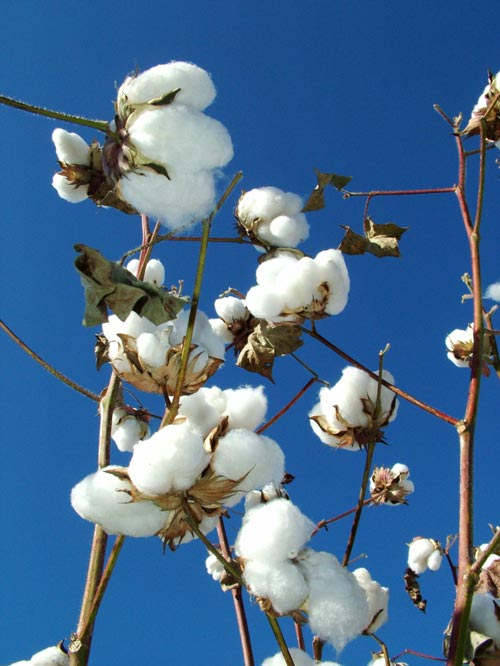
\includegraphics[scale=0.25]{./figure2/defoliation}
      \end{figure}
      \vspace{0.2cm}
    \end{column}
    \begin{column}{0.6\textwidth}
      {\bf Aim:} to assess the effects of five defoliation levels on the
      bolls produced at five growth stages.\\[0.2cm]
      {\bf Design:} factorial 5 $\times$ 5, with 5 replicates.\\[0.2cm]
      {\bf Experimental unit:} a plot with 2 plants.\\[0.2cm]
      {\bf Factors:} Artificial defoliation (\texttt{des}) and
      Growth stage (\texttt{est}).\\[0.2cm]
      {\bf Response variable:} Total number of cotton bolls;\\[0.2cm]
      {\bf Linear predictor:} Following \citet{Zeviani2014},
      $\log(\mu_{ij}) = \beta_0 + \beta_{1j} \textrm{def}_i + \beta_{2j}
      \textrm{def}_i^2$
    \end{column}
  \end{columns}
\end{frame}

\begin{frame}{Parameter estimates}

  \vspace{-0.6cm}
\begin{table}[!ht]
\centering \footnotesize
\caption{Parameter estimates (Est) and ratio between estimate and
  standard error (SE).}
\vspace{-0.5cm}
\label{tab:coef-cotton}
\begin{tabular}{lrrrrrrrr}
  \toprule
  & \multicolumn{2}{c}{Poisson} &
    \multicolumn{2}{c}{COM-Poisson} &
    \multicolumn{2}{c}{COM-Poisson$_\mu$} &
    \multicolumn{2}{c}{Quasi-Poisson} \\
\cmidrule(lr){2-3} \cmidrule(lr){4-5} \cmidrule(lr){6-7} \cmidrule(lr){8-9}
% latex table generated in R 3.4.4 by xtable 1.8-2 package
% Tue Jun 26 13:34:54 2018
 & Est & Est/SE & Est & Est/SE & Est & Est/SE & Est & Est/SE \\
  \midrule
  \rowcolor{col!30}
$\phi, \sigma$ &  &  & 1.585 & 12.417 & 1.582 & 12.392 & 0.241 &  \\
  $\beta_0$ & 2.190 & 34.572 & 10.897 & 7.759 & 2.190 & 74.640 & 2.190 & 70.420 \\
  $\beta_{11}$ & 0.437 & 0.847 & 2.019 & 1.770 & 0.435 & 1.819 & 0.437 & 1.726 \\
  $\beta_{12}$ & 0.290 & 0.571 & 1.343 & 1.211 & 0.288 & 1.223 & 0.290 & 1.162 \\
  $\beta_{13}$ & $-$1.242 & $-$2.058 & $-$5.750 & $-$3.886 & $-$1.247 & $-$4.420 & $-$1.242 & $-$4.192 \\
  $\beta_{14}$ & 0.365 & 0.645 & 1.595 & 1.298 & 0.350 & 1.328 & 0.365 & 1.314 \\
  $\beta_{15}$ & 0.009 & 0.018 & 0.038 & 0.035 & 0.008 & 0.032 & 0.009 & 0.036 \\
  $\beta_{21}$ & $-$0.805 & $-$1.379 & $-$3.725 & $-$2.775 & $-$0.803 & $-$2.961 & $-$0.805 & $-$2.809 \\
  $\beta_{22}$ & $-$0.488 & $-$0.861 & $-$2.265 & $-$1.805 & $-$0.486 & $-$1.850 & $-$0.488 & $-$1.754 \\
  $\beta_{23}$ & 0.673 & 0.989 & 3.135 & 2.084 & 0.679 & 2.135 & 0.673 & 2.015 \\
  $\beta_{24}$ & $-$1.310 & $-$1.948 & $-$5.894 & $-$3.657 & $-$1.288 & $-$4.095 & $-$1.310 & $-$3.967 \\
  $\beta_{25}$ & $-$0.020 & $-$0.036 & $-$0.090 & $-$0.076 & $-$0.019 & $-$0.074 & $-$0.020 & $-$0.074 \\
   \specialrule{0.01em}{0.3em}{0.3em}
 $\ell(\hat{\bm{\theta}})$ & \multicolumn{2}{c}{$-255.803$} & \multicolumn{2}{c}{$-208.250$} & \multicolumn{2}{c}{$-208.398$} & \multicolumn{2}{c}{$  -$}\\
 {\scriptsize AIC} & \multicolumn{2}{c}{$533.606$} & \multicolumn{2}{c}{$440.500$} & \multicolumn{2}{c}{$440.795$} & \multicolumn{2}{c}{$  -$}\\
 {\scriptsize BIC} & \multicolumn{2}{c}{$564.718$} & \multicolumn{2}{c}{$474.440$} & \multicolumn{2}{c}{$474.735$} & \multicolumn{2}{c}{$  -$} \\
 \bottomrule
\end{tabular}
\end{table}
\end{frame}

\begin{frame}{Fitted curves}

\begin{figure}[!htb]

{\centering \includegraphics[width=\textwidth]{figure2/pred-cotton-1} 

}

\caption[Scatterplots of the observed data and curves of fitted values with 95\% confidence intervals as functions of the defoliation level for each growth stage]{Scatterplots of the observed data and curves of fitted values with 95\% confidence intervals as functions of the defoliation level for each growth stage.}\label{fig:pred-cotton}
\end{figure}



\end{frame}

\begin{frame}{Additional results}
  \small
  To compare the computational times on the two parametrizations we
  repeat the fitting 50 times.
  \vspace{-0.2cm}

\begin{figure}[!htb]

{\centering \includegraphics[width=0.95\textwidth]{figure2/comp-times-1} 

}

\caption[Computational times to fit the models under original and reparametrized versions based on the fifty repetitions]{Computational times to fit the models under original and reparametrized versions based on the fifty repetitions.}\label{fig:comp-times}
\end{figure}



\end{frame}

\begin{frame}{Concluding remarks}

  {\bf Summary}
  \begin{itemize}
    \item COM-Poisson is a suitable choice for these situations;
    \item The proposed reparametrization, COM-Poisson$_\mu$ has some
      advantages:
      \begin{itemize}
        \item Simple transformation of the parameter space;
        \item Leads to the orthogonality of the parameters (seen
          empirically);
        \item Full parametric approach;
        \item Empirical correlation between the estimators was
          practically null;
        \item Faster for fitting;
        \item Allows interpretation of the coefficients directly.
      \end{itemize}
  \end{itemize}

  {\bf Future work}
  \begin{itemize}
    \item Simulation study to assess model robustness against
      distribution miss specification;
    \item Assess theoretical approximations for $Z(\lambda, \nu)$
      (or $Z(\mu, \phi)$), in order to avoid the selection of sum's
      upper bound.
  \end{itemize}
\end{frame}

\section{Double COM-Poisson models}

\begin{frame}{Standard regression models}

\textbf{Generalized Linear Models} (GLM) \citep{Nelder1972}:\\[0.1cm]

Let $(y_i, \bm{x}_i)$ a cross-section data set where $y_i's$ are iid
realizations of $Y_i$ according to the exponential family (\text{EF})
distribution. The GLM is specified as follow
$$
  \begin{gathered}
    Y_i \sim \text{EF}(\mu_i, \sigma)\\
    g(\mu_i) = \bm{x}_i^\top \bm{\beta}
  \end{gathered} \quad \Longrightarrow \quad
  \begin{aligned}
    &\text{E}(Y_i)=\mu_i\\
    &\text{Var}(Y_i)=\sigma V(\mu_i).
  \end{aligned}
$$
\vspace{0.3cm}

\textbf{Main limitations}
\begin{itemize}
    \item The exponential family is often restrictive (variance
      function);
    \item The only choice for count data analysis is the Poisson
      distribution;
    \item Only the mean parameter is allowed to depend on covariates
      \citep{Smyth1998}.
\end{itemize}
\end{frame}

\begin{frame}{Regression models for mean and dispersion}

\textbf{Double COM-Poisson regression models (DCMP)}\\[0.1cm]

Let $(y_i, \bm{x}_i, \bm{z}_i)$ a data set where $y_i's$ are iid
realizations of $Y_i$ according to the COM-Poisson distribution
distribution and $\bm{x}_i$ and $\bm{z}_i$ are sub-vectors of the
covariates vector. The DCMP is specified as follow
$$
  Y_i \sim \text{CMP}_\mu(\mu_i, \nu_i), \quad \text{where} \quad
  g(\mu_i) = \bm{x}_i^\top \bm{\beta} \quad \text{and} \quad
  g(\nu_i) = \bm{z}_i^\top \bm{\gamma}.
$$
\vspace{-0.1cm}

\textbf{Log-likelihood function}\\[-0.4cm]
$$
\ell(\bm{\beta}, \bm{\gamma} ; \bm{y}) = \sum_{i=1}^{n} \left \{
  \nu_i\log \left ( \mu_i + \frac{\nu_i-1}{2\nu_i}\right ) -
  \nu_i \log(y_i) - \log[Z(\mu_i, \nu_i)],
\right \}
$$
where $\mu_i = g^{-1}(\bm{x}_i^\top \bm{\beta})$ and
$\nu_i = g^{-1}(\bm{z}_i^\top \bm{\gamma})$
\end{frame}

\begin{frame}{Estimation and inference}

\begin{itemize}
  \item Parameters estimates are obtained by numerical maximization
    of the log-likelihood function (by BFGS algorithm)
  \item Standard errors for regression coefficients (for mean and
    dispersion) are obtained based on the observed information matrix:\\
    {\small $\bm{V}_{\beta \mid \gamma} = \bm{V}_{\beta} -
     (\bm{V}_{\beta, \gamma} \bm{V}_{\gamma}^{-1})^\top
     \bm{V}_{\beta, \gamma}\;$ and
    $\;\bm{V}_{\gamma \mid \beta} = \bm{V}_{\gamma} -
     (\bm{V}_{\gamma, \beta} \bm{V}_{\beta}^{-1})^\top
     \bm{V}_{\gamma, \beta}$}.
\end{itemize}
\vspace{0.5cm}

Strategies
\begin{itemize}
  \item \textbf{Joint:} Estimate
  $(\hat{\bm{\beta}}^\top, \hat{\bm{\gamma}}^\top)^\top$ using the
  complete log-likelihood function;
  \item \textbf{Fixed:} Set the $\hat{\bm{\beta}}$ in the Poisson MLE,
  estimate $\bm{\gamma}$ (with fixed $\bm{\beta}$) and then estimate
  the Hessian matrix for
  $(\hat{\bm{\beta}}^\top, \hat{\bm{\gamma}}^\top)^\top$.
\end{itemize}
\end{frame}

\begin{frame}{Analysis of nitrofen data}
  \begin{columns}
    \begin{column}{0.35\textwidth}
      \begin{figure}
        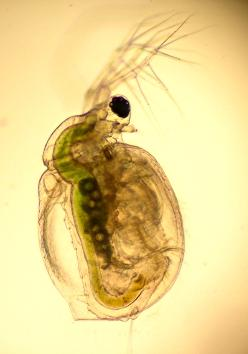
\includegraphics[width=4cm]{./figure2/zooplankton}
      \end{figure}
      \vspace{0.2cm}
    \end{column}
    \begin{column}{0.65\textwidth}
      {\bf Aim:} measure the reproductive toxicity of the herbicide
      nitrofen on a species of zooplankton
      (\textit{Ceriodaphnia dubia});\\[0.2cm]
      {\bf Design:} completely randomized design, with 10
      replicates;\\[0.2cm]
      {\bf Experimental unit:} zooplankton animal;\\[0.2cm]
      {\bf Factor:} Herbicide nitrofen dose (\texttt{dose});\\[0.2cm]
      {\bf Response variable:} Total number of live offspring;\\[0.2cm]
      {\bf Predictors:}
      Cubic to the mean ($\mu$) and linear, quadratic
        and cubic to the dispersion parameter ($\nu$):
    \end{column}
  \end{columns}
\end{frame}

\begin{frame}{Parameter estimates and likelihood ratio tests}
\vspace{-0.5cm}

\begin{table}[ht]
  \centering \scriptsize
  \caption{Estimates and standard errors.}
  \label{tab:coef}\vspace{-0.2cm}
  \begin{tabular*}{\textwidth}{@{\extracolsep{\fill}}crrrr}
    \toprule
    & \multicolumn{4}{c}{Estimate (standard error)} \\
    \cmidrule(lr){2-5}
% latex table generated in R 3.4.4 by xtable 1.8-2 package
% Thu May 24 10:40:34 2018
\multicolumn{1}{c}{Parameter} & \multicolumn{1}{c}{Constant} & \multicolumn{1}{c}{Linear} & \multicolumn{1}{c}{Quadratic} & \multicolumn{1}{c}{Cubic} \\
  \midrule
$\beta_0$ &  2.981 (0.035)$^\text{a}$ &  2.978 (0.042)$^\text{a}$ &  2.972 (0.049)$^\text{a}$ &  2.975 (0.047)$^\text{a}$ \\
  $\beta_1$ & $-$3.952 (0.287)$^\text{a}$ & $-$3.980 (0.365)$^\text{a}$ & $-$4.041 (0.447)$^\text{a}$ & $-$4.013 (0.418)$^\text{a}$ \\
  $\beta_2$ & $-$2.131 (0.260)$^\text{a}$ & $-$2.161 (0.311)$^\text{a}$ & $-$2.218 (0.351)$^\text{a}$ & $-$2.197 (0.330)$^\text{a}$ \\
  $\beta_3$ & $-$0.543 (0.221)$^\text{a}$ & $-$0.573 (0.212)$^\text{a}$ & $-$0.604 (0.206)$^\text{a}$ & $-$0.597 (0.195)$^\text{a}$ \\
   \specialrule{0.0em}{0.2em}{0.3em}
$\gamma_0$ & 0.048 (0.205)\textcolor{white}{$^\text{a}$} &  0.295 (0.211)\textcolor{white}{$^\text{a}$} &  0.243 (0.259)\textcolor{white}{$^\text{a}$} &  0.353 (0.227)\textcolor{white}{$^\text{a}$} \\
  $\gamma_1$ & \multicolumn{1}{c}{$-$} & $-$5.244 (1.363)$^\text{a}$ & $-$7.013 (2.307)$^\text{a}$ & $-$5.729 (1.844)$^\text{a}$ \\
  $\gamma_2$ & \multicolumn{1}{c}{$-$} & \multicolumn{1}{c}{$-$} & $-$3.984 (2.444)\textcolor{white}{$^\text{a}$} & $-$2.918 (1.904)\textcolor{white}{$^\text{a}$} \\
  $\gamma_3$ & \multicolumn{1}{c}{$-$} & \multicolumn{1}{c}{$-$} & \multicolumn{1}{c}{$-$} &  1.522 (1.412)\textcolor{white}{$^\text{a}$} \\

    \bottomrule
  \end{tabular*}
  \\ \vspace{-0.0cm}
  \tiny \raggedright Est (EP)$^\text{a}$ indicates
  $|$Est$/$EP$|$ $> 1,96$.
\end{table}
\vspace{-0.5cm}

\begin{table}[ht]
  \centering \scriptsize
  \caption{Model fit measures and comparisons.}
  \label{tab:anova}\vspace{-0.2cm}
  \begin{tabular*}{\textwidth}{@{\extracolsep{\fill}}lcccrl}
    \toprule
% latex table generated in R 3.4.4 by xtable 1.8-2 package
% Thu May 24 10:40:35 2018
 & D.f & Deviance & AIC & $\rchi^2$ & $\Pr(>\rchi^2$) \\
  \midrule
Constant & 45 & 288.127 & 298.127 & \multicolumn{1}{c}{$-$} & \multicolumn{1}{c}{$-$} \\
  Linear & 44 & 274.111 & 286.111 & 14.0163 & 0.0002 \\
  Quadratic & 43 & 270.493 & 284.493 & 3.6179 & 0.0572 \\
  Cubic & 42 & 269.503 & 285.503 & 0.9898 & 0.3198 \\
   \bottomrule

  \end{tabular*}
\end{table}
\end{frame}

\begin{frame}{Fitted mean and dispersion values}

\begin{figure}[!htb]

{\centering \includegraphics[width=\textwidth]{figure2/fit-values-1} 

}

\caption[(a) Fitted values and confidence bands of 95\% for de dispersion and (b) mean and variances obtained from the fitted model]{(a) Fitted values and confidence bands of 95\% for de dispersion and (b) mean and variances obtained from the fitted model.}\label{fig:fit-values}
\end{figure}



\end{frame}

\begin{frame}{Comparison of the strategies for fitting}
\vspace{-0.2cm}

\begin{figure}[!htb]

{\centering \includegraphics[width=0.8\textwidth]{figure2/compare-strategies-1} 

}

\caption[Comparison of (a) maximized likelihoods, estimates and standard errors and (b) computational times]{Comparison of (a) maximized likelihoods, estimates and standard errors and (b) computational times.}\label{fig:compare-strategies}
\end{figure}


\end{frame}

\begin{frame}{Concluding remarks}
  \textbf{Summary}
  \begin{itemize}
  \item We show how to allow mean and dispersion parameters to depend
    on covariates in the COM-Poisson regression model;;
  \item Estimation and inference can be done based on the likelihood
    paradigm;
  \item Using the orthogonality property in the fixed strategy for
    fitting is faster.
  \end{itemize}
  \vspace{0.5cm}
  \textbf{Current work}
  \begin{itemize}
    \item Perform a simulation study to evaluate estimators properties;
    \item Compare the results with others approaches, DGLM's
      \citep{Lee2006} and GAMLSS \citep{Rigby2005}.
  \end{itemize}
\end{frame}

\section{Flexible mixed models for count data}

\begin{frame}{Motivation}

  Collection of correlated data is very common. \citet{Molenberghs2005}
  use this term in a generic sense to:
  \begin{itemize}
    \item Multivariate observations;
    \item Clustered data or design;
    \item Repeated measurements;
    \item Longitudinal data; and
    \item Spatially correlated data.
  \end{itemize}
  \vspace{0.2cm}

  Some well-known approaches to the analysis of this kind of data:
  \begin{itemize}
    \item Generalized linear mixed models \citep{Breslow1993};
    \item Generalized estimating equations \citep{Liang1986}.
  \end{itemize}
  \vspace{0.2cm}

  Statistical challenge:
  \begin{itemize}
    \item Following a random effects approach, allow the marginal
      distribution of the count data to be over- or underdispersed.
  \end{itemize}
\end{frame}

\begin{frame}{Model specification}
  \small
  Consider a cross-section data set $(y_{ij}, \bm{x}_{ij})$ of a
  repeated measure design, where $y_{ij}$ is the observed count for
  $i$-th group and $j$-th repetition.

  The flexible mixed model is hierarchically specified,
  $$
  \begin{gathered}
    Y_{ij} \mid \bm{b}_{j} \sim \text{FF}(\mu_{ij}, \phi)\\
    g(\mu_{ij}) = \bm{x}_{ij}^\top \bm{\beta} +
    \bm{z}_{ij}^\top \bm{b}_{i}\\
    \bm{b}_i  \sim  \mathcal{N}(\bm{0}, \bm{\Sigma}),
  \end{gathered}
  $$
  where
  \begin{itemize}
  \item where $\text{FF}$ is a flexible family of distributions, like
    COM-Poisson and Gamma-Count distributions;
  \item $\bm{x}_{ij}$ and $\bm{z}_{ij}$ are known vectors representing
    the fixed and random effects, respectively; and
  \item $\bm{\theta} = (\phi, \bm{\beta}, \bm{\Sigma})$ are the unknown
    parameters to be estimated.
  \end{itemize}
\end{frame}

\begin{frame}{Estimation and inference}
  \small
  The likelihood function for the flexible mixed model is given by
  \begin{equation*}
    \label{eqn:likelihood}
    \mathcal{L}(\bm{\theta} \mid \bm{y}) =
    \prod_{i=1}^N \int \prod_{j=1}^{n_i}
    \Pr(Y_{ij} = y_{ij} \mid \bm{b}_{i})
    \left | 2\pi\Sigma \right |^{-\frac{1}{2}}
    \exp \left ( -\frac{1}{2} \bm{b}_i^\top
      \Sigma^{-1} \bm{b}_i \right ) d \bm{b}_i^\top.
  \end{equation*}

  \begin{itemize}
  \item \textbf{Maximum likelihood based}:\\
    Find $\hat{\bm{\theta}}$ such that
    $\mathcal{L}(\hat{\bm{\theta}} \mid \bm{y}) =
    \max [\mathcal{L}(\bm{\theta} \mid \bm{y} )]\,
    \forall \; \bm{\theta} \in \Theta.$ (automatic differentiation,
    expectation-maximization, etc.)
  \item \textbf{Bayesian approach}:\\
    State your prior knowledge about the parameters $\bm{\theta}$, by
    means of probability distributions (prior distributions
    $\pi(\bm{\theta})$); \\[0.1cm]
    Obtain the a posteriori distribution
    $\pi(\bm{\theta} \mid \bm{y}) \propto \mathcal{L}(\hat{\bm{\theta}}
    \mid \bm{y}) \pi(\bm{\theta})$,
    which represents all your knowledge about.\\[0.1cm]
    Often Bayesian inference is performed based on samples of the
    posterior distribution (Gibbs sampler, Metropolis-Hastings, etc.)
  \end{itemize}
\end{frame}

\begin{frame}[fragile]{Implementation on BUGS language}
\vspace{-0.4cm}
\begin{knitrout}\scriptsize
\definecolor{shadecolor}{rgb}{0.122, 0.188, 0.282}\color{fgcolor}\begin{kframe}
\begin{alltt}
model \{
\hlcom{  # Likelihood}
  \hlkwd{for} (i in 1:n) \{
    t[i] <- \hlkwd{exp}(o[i])
    ll[i] <- \hlkwd{log}(\hlkwd{pgamma}(t[i], y[i] * alpha, kappa[i]) -
                 \hlkwd{pgamma}(t[i], (y[i] + 1) * alpha, kappa[i]))
    \hlkwd{log}(kappa[i]) <- gama + X[i, ] %*% beta[] + Z[i, ] %*% b[1:k, g[i]]
    ze[i] ~ \hlkwd{dpois}(-ll[i])
  \}
\hlcom{  # Random effects}
  \hlkwd{for} (i in 1:l) \{
    b[1:k, i] ~ \hlkwd{dmnorm}(\hlkwd{rep}(0, k), Tau)
  \}
\hlcom{  # Prioris}
  Tau ~ \hlkwd{dwish}(R_ranef, df_ranef)
  Sigma <- \hlkwd{inverse}(Tau)
  gama ~ \hlkwd{dnorm}(0.0, tau_gama)
  alpha <- \hlkwd{exp}(gama)
  \hlkwd{for} (i in 1:p) \{
    beta[i] ~ \hlkwd{dnorm}(0.0, tau_beta)
  \}
\}
\end{alltt}
\end{kframe}
\end{knitrout}
\end{frame}

\begin{frame}[fragile]{Implementation on BUGS language}
\vspace{-0.4cm}
\begin{knitrout}\scriptsize
\definecolor{shadecolor}{rgb}{0.122, 0.188, 0.282}\color{fgcolor}\begin{kframe}
\begin{alltt}
model \{
\hlcom{  # Likelihood}
  \hlkwd{for} (i in 1:n) \{
     lambda[i] <- (mu[i] + (nu - 1)/(2 * nu))^nu
     \hlkwd{for} (j in 1:sumto) \{
      K[i, j] <- \hlkwd{exp}(j * \hlkwd{log}(lambda[i]) - nu * \hlkwd{logfact}(j))
    \}
    ll[i] <- y[i] * \hlkwd{log}(lambda[i]) - nu * \hlkwd{logfact}(y[i]) - \hlkwd{log}(\hlkwd{sum}(K[i, ]))
    \hlkwd{log}(mu[i]) <- X[i, ] %*% beta[] + Z[i, ] %*% b[1:k, g[i]] + o[i]
    ze[i] ~ \hlkwd{dpois}(-ll[i])
  \}
\hlcom{  # Random effects}
  \hlkwd{for} (i in 1:l) \{
    b[1:k, i] ~ \hlkwd{dmnorm}(\hlkwd{rep}(0, k), Tau)
  \}
\hlcom{  # Prioris}
  Tau ~ \hlkwd{dwish}(R_ranef, df_ranef)
  Sigma <- \hlkwd{inverse}(Tau)
  phi ~ \hlkwd{dnorm}(0.0, tau_phi)
  nu <- \hlkwd{exp}(phi)
  \hlkwd{for} (i in 1:p) \{
    beta[i] ~ \hlkwd{dnorm}(0.0, tau_beta)
  \}
\}
\end{alltt}
\end{kframe}
\end{knitrout}
\end{frame}

\section{Work resulting}

\begin{frame}{Academic contributions}

  \begin{enumerate}
  \item Reparametrization of COM-Poisson models:
    \begin{itemize}
      \setlength{\itemindent}{-0.4cm}
    \item Oral presentation at 62\textsuperscript{a} RBras /
      17\textsuperscript{o} SEAGRO (2017)\\
      \url{https://github.com/jreduardo/rbras2017}.
    \item Submitted article (2018) \textit{``Reparametrization of
        COM-Poisson Regression Models with Applications in the
        Analysis of Experimental Data''}\\
      \url{https://arxiv.org/abs/1801.09795}.
    \end{itemize}
  \item Probabilistic models for count data:
    \begin{itemize}
      \setlength{\itemindent}{-0.4cm}
    \item Oral presentation at 63\textsuperscript{a} RBras (2018)\\
      \url{https://github.com/jreduardo/rbras2018b}.
    \end{itemize}
  \item Double COM-Poisson models:
    \begin{itemize}
      \setlength{\itemindent}{-0.4cm}
    \item Oral presentation at 63\textsuperscript{a} RBras (2018)\\
      \url{https://github.com/jreduardo/rbras2018}.
    \end{itemize}
  \end{enumerate}
  \vspace{0.3cm}
  \textbf{Work in progress...}
  \vspace{0.4cm}
\end{frame}

\section*{Bibliography}
\begin{frame}[allowframebreaks, t]{References}
  \footnotesize
  \vspace*{-0.5cm} \nocite{RibeiroJr2018}
  \bibliography{../bibliography.bib}
\end{frame}

\section*{}
\begin{frame}[plain, noframenumbering]
  \centering
  \textcolor{col}{\Huge Thank you!}\\[0.5cm]
  \url{jreduardo@usp.br}\\
  \url{www.leg.ufpr.br/~eduardojr}
\end{frame}

\end{document}
